\pagebreak

\section*{Q1}
\begin{solution}[\textbf{2}]
\hfill\break
\textbf{a)} First we show that if $u$ is a solution to $u_t +  uu_x = 0$, then $w = u^2$ is a smooth solution of $(2)$. 
\begin{align*}
    u_t + uu_x &= 0 \\
    (2u)u_t + (2u)u_x &= 0 \\
    2uu_t + 2uu_x &= 0 \\
    \left(u^2\right)_t + \left(\frac{2}{3} (u^2)^{\frac{3}{2}}\right)_x &= 0 \ \ \text{Since $u$ is smooth.} \\
    w_t + \left(\frac{2}{3} w ^{\frac{3}{2}}    \right)_x &= 0
\end{align*}
In the other direction, we start with $w = u^2$ as a solution to $w_t + \left(\frac{2}{3}w^{\frac{3}{2}}\right)_x  = 0$.
\begin{align*}
    w_t + \left(\frac{2}{3}w^{\frac{3}{2}}\right)_x &= 0 \\
    (u^2)_t + \left(\frac{2}{3}u^{3}\right)_x &= 0 \\
    2uu_t + 2u^2u_x &= 0 \ \ \text{Since $u$ is smooth.} \\
    2u(u_t + uu_x) &= 0
\end{align*}
Thus we have two cases. If $u = 0$, then trivially, $(1)$ holds. Otherwise if $u > 0$, then we can divide by $2u$ giving us that,
\begin{align*}
u_t + uu_x = 0
\end{align*}
as required. This concludes the proof in both directions.
\hfill\break
\hfill\break
\textbf{b)}  Figures can be added as follows:
\begin{figure}[H]
    \centering
    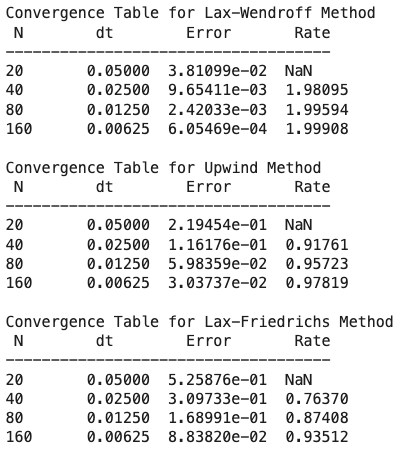
\includegraphics[scale=0.35]{./figures/q2-table.png}
\end{figure}
\end{solution}

